\section{Lifehacks?!}
\begin{epigraph}
    --- Чему равен объём пиццы радиусом z и высотой a?\\
    --- \( \pi\cdot z\cdot z\cdot a \)!
\end{epigraph}

\noindent\emph{If you have a good lifehacks, then you had a something fucks.}

\noindentИдеи для лайфхаков:
\begin{itemize}
    \item Если вам лень убирать квартиру к приходу гостей, просто покажите им ваш срач и задайте меланхолично вопрос: "Что же автор хотел этим сказать?" \emph{(Осторожно: есть опасность стать художником!)}
    \item Аналогично можно объяснить любую странность вашего поведения: "Я художник, я так вижу!"
    \item Если вы хотите что-то сделать, то возьмите выпейте чашку крепкого чая с долькой лимона/лайма и большим бутербродом. Теперь вы бодры и полны энергии! Просто сделайте задуманное)
    \item Если вам никак не удаётся уснуть -- займитесь делом, которое постоянно откладываете. При определённом уровне тренировки ваша лень поборет бессонницу, и вы за\emph{zzz}нёте...
    \begin{figure}[ht!]
        \centering
        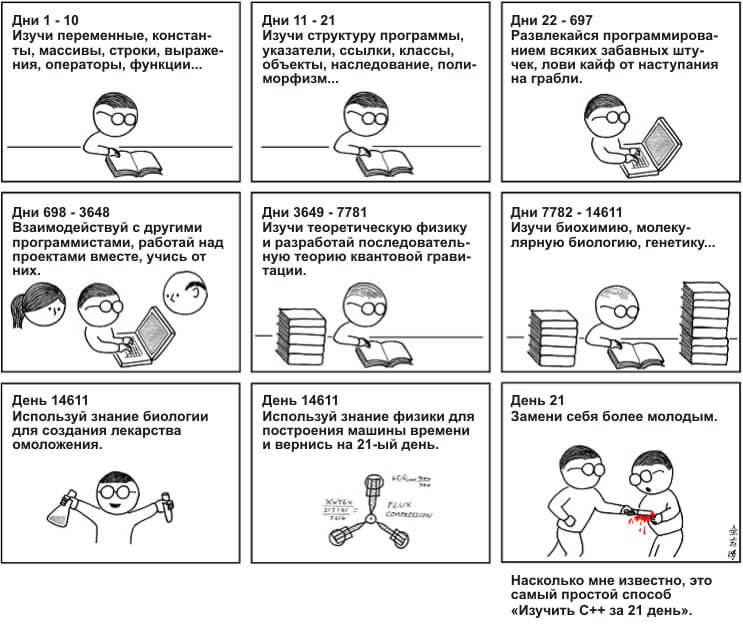
\includegraphics[width=0.75\textwidth]{c++21day}
    \end{figure}
    \item Если у вас возникло желание начать бороться со своей ленью, остановитесь, прислушайтесь к себе: а не лень ли вам бороться с ленью?\\
        Нет -- тогда расслабьтесь. Ваш уровень лени ниже критического.\\
        Да -- тогда нужно...а ну на фиг -- мне лень дописывать этот лайфхак
\end{itemize}

\newpage

\noindentЛайфхаки от К.О.:
\begin{itemize}
    \item Чемодан в поездку можно собрать значительно быстрее, если его не разбирать из предыдущей.
    \item Длительный перелёт/переезд поможет скоротать какое-нибудь увлекательное занятие. Например, сон.
    \item Если вы, как писатель/издатель, хотите \\ добиться того, чтобы ваш текст \\
        прочитывали полностью и \\
        не пропускали слова, \\
        то располагайте \\
        его в виде \\
        буквы \\
        F.
\end{itemize}